\section{Introduction and Motivation}
\label{sec:intro}

\begin{figure*}[hb]
  \centering

  \begin{subfigure}[t]{0.42\tw}\centering
    \includegraphics[width=\textwidth]{no-revocation.svg.pdf}
    \caption{Stock Mesos -- No Revocation}
    \label{fig:wo-revocation}
  \end{subfigure}%
  \hfill
  \begin{subfigure}[t]{0.42\tw}\centering
    \includegraphics[width=\textwidth]{revocation.svg.pdf}
    \caption{Mesos With Revocation}
    \label{fig:w-revocation}
  \end{subfigure}%

  \caption{\textbf{Comparison of Mesos With and Without Revocation Enabled}
  Example Mesos cluster with two slots. Both example frameworks have two parallel tasks so they are able
  to fully utilize the entire cluster. Framework 2 arrives later than the Framework 1. Yellow bars
  corrrespond to the time that the framework has to wait for an offer from Mesos. Red bar corresponds
  to the time that framework is running a task on a node.
  }
  \label{fig:revocation}
\end{figure*}


As the data analytics and processing needs of companies grow, systems designers are looking
more and more to using clusters in order to provide for those needs. Clustering of compute
resources permits more efficient allocation of compute resources to tasks relative to
na\"{\i}ve static partitioning by allowing unused resources to quickly and easily be shared for
use by other tasks. This lets companies to more effectively deal with dynamic workloads by
giving compute clients the ability to pickup or shed resources in time as their computational
requirements shift. For example, during the day a retailer has to devote substantive processing
power to ensure all transactions are completed in a timely manner such that the retailer can do
real business. However, during the evening when transaction loads are light, the excess
resources are better spent doing data analysis on the transaction data to track buying trends
and better inform managers for making business decisions. These clusters need specific cluster
management software that maps compute nodes to clients and provides administrators a convenient
point to monitor the status and utilization of all agents in the system.

\subsection{Apache Mesos}
Apache Mesos is one such cluster manager that was originally developed by the UC Berkeley AMP
Lab and is currently in use to manage clusters at Twitter and Conviva [1,2 REF]. Mesos uses an
event-driven architecture and is written in C++ and built on top of the Libprocess and
Zookeeper libraries. This paper will explain enough of the Mesos architecture to understand the
change implemented in the project; however, please refer to the original paper [1] for the
particular details on other parts of the system. The Mesos API model does not require
frameworks to specify the fine details of what resources the participating frameworks (the
clients) need.  Rather, Mesos compiles a listing of available resources at nodes into an offer
that it then presents to a framework. The framework may then analyze the resources in the offer
and then cherry-pick the specific nodes onto which Mesos should launch new tasks for the
framework. This allows frameworks to fulfill arbitrarily complex resource allocation
requirements without complicating the Mesos scheduler. For example, by tracking its previous
allocations, frameworks could ensure its tasks are all located on the same rack in the system
(for better IPC speed) or far away from each other (for better resiliency to failure), only
launched on nodes with internet access (for webservers), or, for Hadoop-like tasks,
preferentially launched on nodes already containing the data to be processed (to minimize data
fetch time). To enforce fairness amongst all frameworks, the allocator in Mesos implements
dominant resource fairness [3 REF] and only makes new offers to frameworks in order of
increasing dominant share. Over time, this is expected to balance out the system amongst all
frameworks. Mesos has been found to be highly scalable (up to 50000 nodes) and competitive when
run against static partitioning for various Hadoop and Spark workloads.

\subsection{Fairness Problems with Mesos}
Producing fairness by ordering offers to frameworks, unfortunately, does not work in the
general case. The original evaluation of Mesos focused on MapReduce or MapReduce-like jobs,
which are generally characterized by having a small footprint and, critically, low execution
times. Thus, for any small interval of time during those tests, tasks were ending thus freeing
up resources on nodes allowing offers to be made to undersubscribed frameworks. However, this
behavior is not guaranteed in general, particularly in systems containing frameworks with
`long' running tasks. Assuming these same frameworks are capable of spawning speculative
execution (in order to avoid letting cluster resources go to waste during times of low
interest), all system resources will be reserved for extended periods of time leaving new
frameworks (or equivalently, other frameworks that suddenly need a bunch of resources to
respond to a workload burst) unable to get resources in a timely manner. These high latencies
may be unacceptable for interactive frameworks that must launch tasks immediately to respond to
user queries.

Implementation details of Mesos also reveal other, more subtle fairness issues that are not
properly resolved by the basic offer model. The resource allocator in Mesos takes a snapshot of
all resources currently allotted to frameworks right as it must decide to whom the offer must
be directed and always selects the one with the lowest dominant share at that instant. Thus, a
framework can arrange to almost always capture the next offer by scheduling all tasks to end
within Mesos' one second scan interval. Since Mesos does not restrict how much of an offer is
taken, the greedy framework is thus able to relaunch onto all the resources currently used up
plus anything else freed during the update. This problem behavior arises more commonly with
frameworks that launch very large resource-heavy tasks (which, again, is in stark contrast to
light MapReduce tasks). Also, in order to avoid race conditions in accepting offers, Mesos will
not simultaneously offer the same resource to different frameworks. Since Mesos generally
includes all available resources when constructing offers, frameworks that take an excessive
period of time deciding on offers will end up wasting those offered resources in a contentious
system.

While admittedly many of these issues would only seem to arise because of a `maliciously'
written framework, many times the difference between buggy or flawed design and malicious
design is merely semantic. For example, an offer response may be inappropriately delayed due to
a framework crash. Alternatively, greedy frameworks may have just been designed to always fill
up large portions of an offer with speculative work under the assumption that the large offer
means the system is unloaded and thus the resources would just to waste otherwise. Thus, even
for completely closed deployments of Mesos, resolving these issues will lead to a more stable
overall design. 

\section{Proposed Solution}
Acknowledging that a core problem with the offer-based fairness solution of Mesos starts
breaking down as the system fills and no resources are available, the clear solution is to
simply revoke resources from `oversubscribed' frameworks in order to make resources available.
Mesos is expected to be run on a cluster composed of somewhat unreliable nodes and thus
frameworks already must be instrumented to cope with tasks failing abruptly. Even so, killing a
task effectively causes what is commonly called `goodput loss' since all time that task had
previously spent with those resources is now effectively lost (although raw system utilization
numbers may be maxed). Also, not all frameworks cope equally well with task-loss. MapReduce
frameworks are able recover very quickly whereas data analysis frameworks using MPI to
synchronize work amongst task processes on different machines may require all participating
tasks to stall (or worse terminate without saving) when one task is lost. These considerations
drive the need for conservative revocations that minimize the amount of revocation done.

Following this goal, this project partly extended the communication model of Mesos to allow
frameworks to send a new type of message indicating resource needs. The documentation for this
message makes a clear distinction between needs and desires by defining needs as the minimum
possible resources that framework requires to function according to its defined specifications
and SLAs. Resources desired for doing speculative execution or merely to get through the task
queue faster are not and must be acquired through traditional means. Mesos administrators are
encouraged to filter these resource need requests to ensure frameworks are making reasonable
demands. The Mesos allocator tracks these demands and periodically checks to ensure all
frameworks have their demand or, altarnatively, enough free resources exist in the system to
cover the needs. If not, Mesos starts revoking tasks from frameworks using resources over their
defined need. In order to minimize goodput loss, Mesos revokes tasks from a framework starting
with the most recently launched task. Frameworks are permitted to adjust their needs over time
(for example, interactive frameworks may relinquish demands for resources when no user queries
are pending) and the system is designed to respond quickly to these changes. MPI-like
frameworks that prefer not to lose tasks can thus insulate themselves from revocation by always
keeping their task resource below their posted resource needs whereas MapReduce-like frameworks
are still able to speculative execute but with the understanding this leaves them open to
revocation and thus higher task-loss rates. The previous issue of frameworks tying up resources
by not responding to offers was resolved by revoking offers from frameworks after an
exponentially expanding timeout period.

Using resource revocation to only satisfy needs and not balance the system reflects the
observation that offer-based DRF was working to balance the system in general only failing due
to latency issues in select scenarios. This also relieves from the Mesos the responsibility of
determining if a resource-light framework would even use resources revoked from a heavier
framework. Whereas offer responses are very specific by detailing precisely which nodes to use
resources on, need requests are by design kept general specifying only quantity of a resource
type needed but not location. This allows Mesos administrators to more easily ensure all needs
for their system are actually satisfiable. Alternative solutions where Mesos submits `tentative
offers' of the whole system to frameworks and then used that response to drive revocation
decisions lead to hard-to-resolve conflicts. For example, a framework would then reply it needs
a resource on a specific node which Mesos then must revoke to provide whereas that request may
have been satisfiable on a different node requiring a less-painful revocation. More nuanced
responses with alternatives could be made but this rapidly complicates the design of Mesos'
simple offer model.

